% Please do not change the document class
\documentclass{scrartcl}

% Please do not change these packages
\usepackage[hidelinks]{hyperref}
\usepackage[none]{hyphenat}
\usepackage{setspace}
\doublespace

% You may add additional packages here
\usepackage{amsmath}
\usepackage{graphicx}
\usepackage{wrapfig}
\graphicspath{ {./images/} }

% Please include a clear, concise, and descriptive title
\title{Market Research} 

% Please do not change the subtitle
\subtitle{COMP240 Market Research}

% Please put your student number in the author field
\author{1507516}

\begin{document}
\maketitle


%\listoftables
%\listoffigures

\section{Introduction}
Firelock is a game being developed by R-LOC Studios. The game is a strategic turn based First Person Shooter (FPS) with a colorful art direction.


\section{Target Market}
The market for strategic turn-based multiplayer shooters is pretty small with only 2 popular games that have similar gameplay mechanics.
These games are Valkryia Chronicles and Frozen Synapse \cite{Valkyria, Frozen}.

 Both these games are fairly popular with Valkryia Chronicles having over 900,000\cite{Valkyria} in sales and Frozen Synapse with just over 700,000 \cite{Frozen}.
 
 There is currently a large market for first person multiplayer games (citation needed).

There is also a large market for turn based strategy games E.g. Xcom 2\cite{xcom} which has almost 1.4M in sales and Sid Meier's Civilization V which has over 10M \cite{civV}. 

%TABLE OF SIMILAR GAMES
\begin{table}
	\begin{tabular}{ |p{4cm}||p{3cm}|p{3cm}|  }
		 \hline
		 \multicolumn{3}{|c|}{\textbf{Similar Games Comparison}} \\
		 \hline
		 \textbf{Game} & \textbf{Total Sales} & \textbf{Price} \\
		 \hline
		 Valkyria Chronicles   & 931,442    &\pounds 14.99\\
		 Frozen Synapse  & 734,572  & \pounds 18.99  \\
		 Verdun  & 623,081  & \pounds 18.99  \\
		 \hline
	\end{tabular}
	\caption{Similar games}
	\label{table:similar}
\end{table}

\section{ Target Audience}
The main Target Audience for this product is people who like games such as Valkyria Chronicles and Frozen Synapse, furthermore those who like to play games with friends.
The demographic for the game would be males and females in the age range of about 12+.

Because the target audience is young and will generally not have a lot of disposable income, the game is priced at \pounds 7.99. This is almost half of what competing games are selling at. (Valkyria Chronicles is \pounds 14.99 and Frozen Synapse is \pounds 18.99) \cite{Valkyria, Frozen}. The reason why the game is priced so low is because we are a new company so we need to build a reputation before being able to charge more.



\section{Finances}
\begin{figure}[h]
	\center{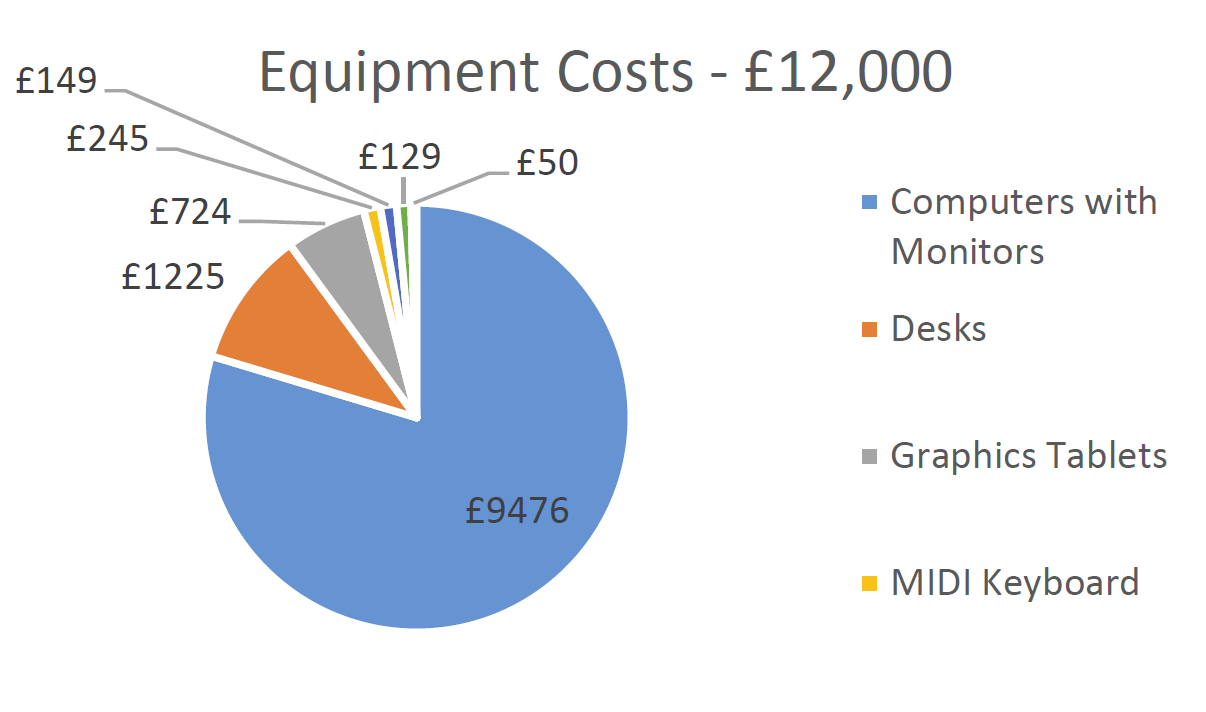
\includegraphics[width=8cm]{Finances}}
	\caption{Equipment Costs	}
\end{figure}

\section{Marketing}
To help market the game R-LOC is planning to target Youtube and Twitch steamers and content creators to help gain interest in the game. 
This is because streamers such as Yogscast have such a large audience they can significantly help the sales of a game \cite{Hoggins, Rose}.  To help encourage steamers to review the game, R-LOC is intending to create 3D models of in game objects, these 3D printed objects can be shipped to a small selection of streamers which will help draw attention to the game. These 3D printed objects can be created cheaply and easily using on-site University 3D printers \cite{Rose}.

Furthermore R-LOC will use the traditional marketing angle of using social media advertising i.e. keeping an active and continually updated web presence. 
This also includes establishing their brand on Facebook and Twitter with regular development updates, this will help involve the community with the development of the game and help keep them invested for a longer period of time.

Humble bundle store take 25\% \cite{HumblebundleFAQ} and steam and GOG take roughly 30\% (Citation needed).

Primary distribution will be on steam.

\section{Conclusion}
In conclusion...


%References steamspy:
%https://steamdb.info/app/98200/graphs/
%https://steamdb.info/app/242860/graphs/
%https://steamdb.info/app/268500/graphs/
%https://steamdb.info/app/294860/graphs/


\bibliographystyle{ieeetr}
\bibliography{comp240-market}

\end{document}
